\documentclass[12pt]{article}
\usepackage[utf8x]{inputenc}
%\usepackage[spanish]{babel}
\usepackage{url}
\usepackage{lipsum}
\usepackage{graphicx}
\usepackage{color}
\usepackage{amsmath}
\usepackage{amssymb}
\usepackage{verbatim}
\usepackage{float}
\usepackage{indentfirst}

\title{
\vspace{-30mm}\begin{figure}[h]
\centering

\includegraphics[width=1.4in]{logoUJM}
\label{escudo}
\end{figure}Data Mining Project Report}
\author{Marco Odehnal\\MLDM}

\begin{document}
\bibliographystyle{ieeetr}
	
\maketitle
\section*{Introduction}
\par{Travelling is said to be one of the biggest pleasures of life and today, there is a great amount of people who have taken a trip to different cities. Airplanes have become the most popular means of transportation when we talk about covering long distances because of their speed, prices and safety controls. However, airplane crashes have become the primary fear of travelers who are not familiar with aircrafts, even though the rate of accident is the lowest, compared to the other means of transportation \cite{bib:crashtransport}.}\\

In the present work, we use data mining techniques in R, in order to gain insights about airplane crashes due to accidents, war and hijacks. We also provide a predictive model for the number of fatalities for the accidents in order to check if the security measures allow to reduce the number of fliers' death. The project is organized according to CRISP-DM framwwork \cite{bib:crisp}: (1) Problem Understanding, (2) Data Understanding, Data Preparation, (4) Modeling, (5) Evaluation, and (6) Deployment.

\section{Problem Understanding}
First, we will study the influence of malicious human behavior (hijack) and war over the airplane crashes. We will see if the casualties and these factors have been controlled throughout the years. We will also compare the odds of survival in the situations of hijack, battle, and regular accidents. The time may also be correlated with the occurrence of crashes.\\

Are we able to survive a place crash? It is natural to believe that there is no way to survive such a crash, but we will provide an answer to this question by using qualitative and quantitative statistical techniques. Finally, we want to generate a predictive model that will allow us to forecast the number of fatalities in aircraft crashes in the following years. 

\section{Data Understanding}
This project used the dataset known as "Historical Plane Crashes", which can be downloaded from \cite{bib:dataset}. All of the observations have been labeled with a date, which makes it interesting for doing time series analysis, and a summary of the crash, which can lead to relevant findings by using text mining techniques.\\

The dataset consideted has 5783 observations, and 13 attributes corresponding to the \textbf{date}, \textbf{time}, \textbf{location}, \textbf{airline operator}, \textbf{flight number}, \textbf{route}, \textbf{aircraft type}, \textbf{registration}, \textbf{fuselage number}, \textbf{people aboard}, \textbf{number of fatalities}, \textbf{gound casualties}, and \textbf{summary of the accident}. The total file size is 2.178 KB.\\

The summary, time and location attributes require the usage of text mining techniques to properly process all the information and therefore, studying in detail these attributes is out of the scope of this work.\\

To be able to properly answer the questions in the Problem Understanding section, we will have to manipulate this dataset, as it is explained in the following section.\\
	
\section{Data Preparation}

We want to consider the three types of airplane crashes: accident, battle, and hijack. In this project we will not be using text mining techniques, however, the only way to separate the split the data into these three classes is by checking the summary of the crashes. The hijacked planes always displayed the word "hijack" in the summary, and the intercepted planes, always displayed "shot down". The remaining observations that did not belong to any of these two classes, were considered accidents. After splitting, we verify that in fact, this criterion induces a partition over the dataset, which means that an observation can only belong to one of these classes.\\

There is no explicit information in the dataset about the survivors, thus, we subtract the fatalities from the number of survivors. The observations with missing values regarding the people aboard were removed from the dataset (only 40 rows omitted).\\

For the time series modeling, we needed to parse the dates and aggregate the values. We transformed the date strings into date format by using the \texttt{parse\_date\_time} from the \texttt{lubridate} package. After this, we created time series of the people aboard, survivors and fatalities by grouping the dates to the values, using the \texttt{zoo} package. We removed the outliers that imbalanced the  \textquotedblleft hijack" and \textquotedblleft shot down" time series. Finally, the time series were considered starting from the year 1930 and, the observations were grouped by four quartiles of the year, taking the mean between the data.

\section{Modeling}

Before selecting a model for forecasting our time series, it is necessary to determine whether it is seasonal or not. If it is true, the series can be decomposed into a trend, seasonal and randomness components in an additive or multiplicative way \cite{bib:shumway2000time}. In this particular problem, the Figure \ref{fig:acFTS} suggests that there is seasonality in the series, since there are many oscillations.\\

\begin{figure}[H]
	\centering
	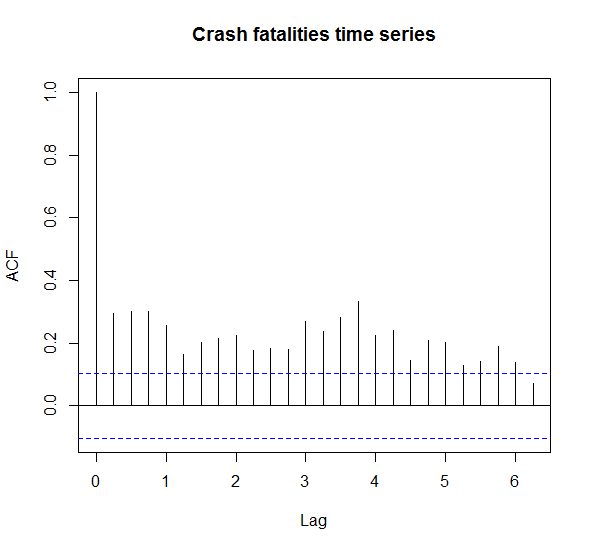
\includegraphics[width=0.8\linewidth]{acfFatalities}
	\caption{Autocorrelation function for the fatalities time series.}
	\label{fig:acFTS}
\end{figure}

In order to provide a good multiplicative time series model, we compare two variations of the Holt-Winters model \cite{bib:forecastingprinciples}. The first one is the multiplicative model for seasonal time series, where we set the parameter associated to the seasonality. The second model is the exponential smoothing by setting both $\gamma,\beta = 0$. We can see in Figure \ref{fig:HoltWinters} that the exponential smoothing explains better the general behavior of the time series, however, the Holt-Winters model exploits the seasonality of the series and attemps to make predictions depending on which period determines the change in behavior. The Holt-Winters seasonal model fits better the data with an SSE error of 9342039, whereas the exponential smoothing achieved an SSE of 9653885; the exponential smoothing is not interesting for predictions, since the predicted values are constant.\\

\begin{figure}[H]
	\centering
	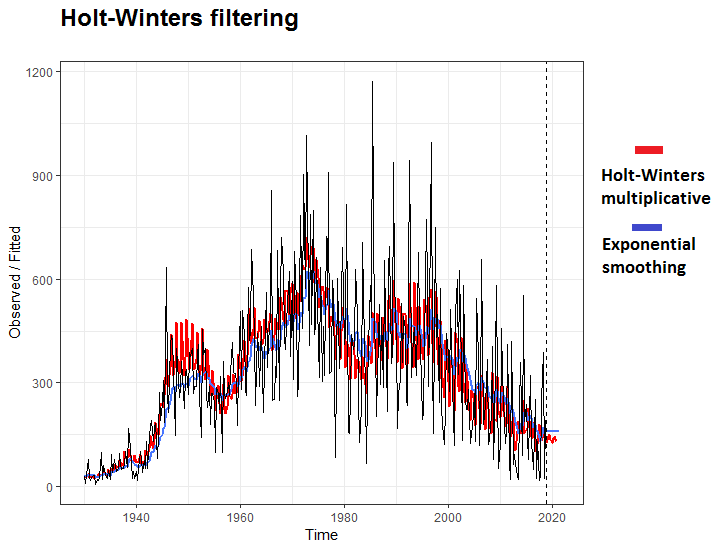
\includegraphics[width=1\linewidth]{holtWinters}
	\caption{Holt-Winters models evaluated over the fatalities time series.}
	\label{fig:HoltWinters}
\end{figure}

The optimal parameters of the Holt-Winters seasonal model are: $$\alpha=0.0784, \beta=0.1,\gamma=0.0751$$

\section{Evaluation}

Travelling by airplane has become widely known as the safest mode of transportation, and this can be confirmed by Figure \ref{fig:numCrash}, in which we can notice that the number of crashes has been decreasing after the year 1990. At the same time, the number of fatalities has been decreasing, as we saw from the time series analysis. In fact, according to the Holt-Winters seasonal model, the number of fatalities from airplane crashes will have decreased 7\% by 2021 (since the predictions of the model in Q4 for 2019 and 2021 yield 140.51 and 130.63 deaths, respectively).\\

\begin{figure}[h]
	\centering
	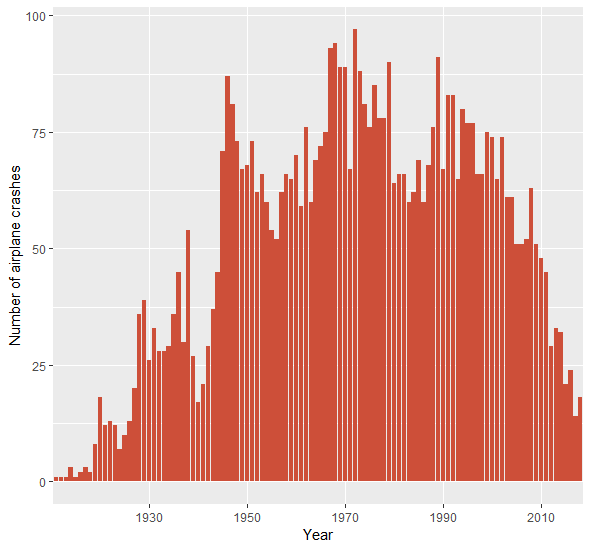
\includegraphics[width=0.8\linewidth]{numCrash}
	\caption{Number of airplane crashes registered from 1908 until 2018.}
	\label{fig:numCrash}
\end{figure}

We can verify that there is no relationship between the time of the year and the airplane crashes, as it is seen in Figure \ref{fig:equalityPlot} (a). Also, we can notice in Figure \ref{fig:equalityPlot}, (b) that people will not always die in crashes, there is an equal chance of survival overall. \\

Hijacks should not be a major concern among the passengers, since only 0.6\% of the airplane crashes were caused by hijacks, and the last tragic events were the 9/11 attacks in 2001. It is normal to believe that there are many airplane crashes caused by war, but only this is only the 2.45\% of all the registered data. 

\begin{figure}[H]
	\centering
	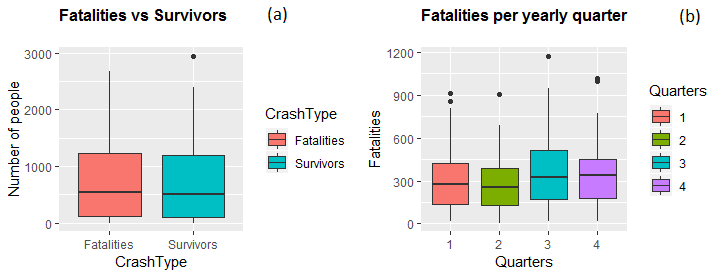
\includegraphics[width=1\linewidth]{boxPlots}
	\caption{Boxplots between different quantities. (a) Boxplot comparison between number of survivors and fatalities. (b) Number of fatalities per yearly quarters.}
	\label{fig:equalityPlot}
\end{figure}

\section{Deployment}

Many experiments were done before obtaining the most meaningful results, and only these tests were considered for the final code. The total running time was \texttt{2.6068} seconds.\\

The world population should be convinced that airplanes are reliable, and statistics makes this statement stronger. Users should have access to this study and R Shiny offers a great way to create a server, which can be deployed in the cloud (either Google Cloud Platform or Amazon Web Services). The deployed code should have a user-friendly interface that allows users to check interactive plots, including time series predictors. 

\section*{Conclusions}

Most datasets have interesting hidden knowledge that requires intuition and creativity. This one is no exeption, because terrorist often "hijack" airplanes and airplanes involved in battle are often "shot down". We discovered that the human being has caused less than 4\% of all crashes and the efforts put into action in order to avoid accidents have made airplane crashes less likely to happen. After the 9/11 attacks, the security improvements managed to prevent airplane crashes caused by terrorists. There is still no world peace, so it is expected that more military planes crash in the future.\\

Datasets may also have time-related data, which can be a hint for using time series models. In this project, we were able to fit a Holt-Winters model that forecasted a decrease in the number of fatalities for the next years. Where should we fly to in the next holidays?


\bibliography{CE}

\end{document}